\chapter{Tracking}%
\label{chap:10}

\section{Fundamental approaches}
Tracking has many application in computer vision, for example tracking people in
a video or tracking dividing cells sequence of microscopy images. The latter
poses a particularly difficult challenge, since here targets (the cells) can
divide and we want to track for each offspring from which cell it has
originated.

We discuss three ``school of thoughts'' for solving such tracking problems. The
first, called \emph{space-time segmentation} we simply treat time as a third
space dimension and apply instance segmentation methods similar to those that we
have discussed in previous chapters.

In the second approach, called tracking-by-assignment or data association, we
first try to detect the objects of interest at each time step individually. If
every time step is processed, we then consider possible associations between the
detected objects in neighbouring time steps (in practice we do not consider all
possible associations since often certain assumptions are made a priori, for
instance we know that cells only move with a certain speed and thus, cells that
are at a certain position at time $t-1$ can only be within a certain region of
this position at time $t$). The last class, which we not discuss in this
lecture, are state-space models such as the Kalman filter or generally hidden
Markov models. In Table~\ref{tab:tracking} we listed some of the advantages and
disadvantages of the three approaches.

\newcommand{\bigplus}{\Large$+$} \newcommand{\bigminus}{\Large$-$}
\begin{table}[htpb]
  \centering { \def\arraystretch{1.2}%
    \tabcolsep=10pt%
    \begin{tabular}{lx{1.5cm}x{1.5cm}x{1.5cm}}
      \toprule
      & \tcirc{1} & \tcirc{2} & \tcirc{3} \\
      \midrule
      Can handle large displacements & \bigplus & \bigplus & \bigplus \\
      Affords joint segmentation and tracking & \bigplus & $+$ & \bigminus \\
      Can handle unknown number of particles & \bigplus & \bigplus & \bigminus \\
      Can handle dividing particles & \bigplus & \bigplus & $+$\\
      Has representation for the internal state & \bigminus & \bigminus & \bigplus \\
      \bottomrule
    \end{tabular}
  }
  \caption{Advantages and disadvantages of space-time segmentation (\tcirc{1}),
    tracking-by-assigment (\tcirc{2}), and state space methods (\tcirc{3}) when
    used for tracking.}%
  \label{tab:tracking}
\end{table}

In all three schools we have a neural network that gets the dense video input
which usually has the same (dense) output dimensions. Often, for instance when
tracking dividing cells, we would rather like a tree that shows how the
different cells and their offsprings behaved and divided over time. That is, we
want a sparse output. This dense to sparse conversion is something that
convolutional neural network often struggle with.

\section{Tracking by association: Min cost flow}
We begin with a simple example of tracking without division (we also assume that
no new detections are born and detections do not die). The detections as
assignments are given for three time steps in Figure~\ref{fig:tracking}. The
second and third image show the detected tracks when matching detections only
between two consecutive frames and when using a shortest path approach,
respectively. We can see that both are not applicable for this task since the
results are not consistent with our assumptions.

\begin{figure}[htpb]
  \centering
  \begin{subfigure}{\textwidth}
    \centering
    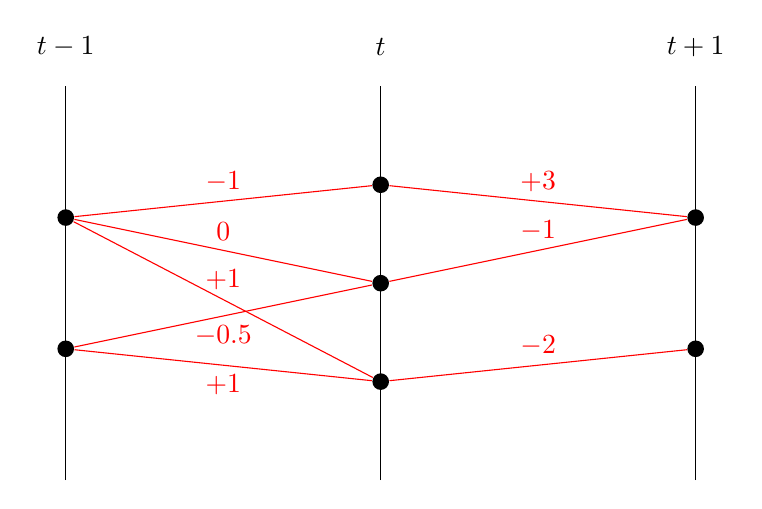
\begin{tikzpicture}
      \draw (0,0) -- (0,5);%
      \draw (4,0) -- (4,5);%
      \draw (8,0) -- (8,5);%

      \node[circle,inner sep=0pt, minimum size=6pt,fill] (A1) at (0,1.6666) {};%
      \node[circle,inner sep=0pt, minimum size=6pt,fill] (A2) at (0,3.3333) {};%

      \node[circle,inner sep=0pt, minimum size=6pt,fill] (B1) at (4,1.25) {};%
      \node[circle,inner sep=0pt, minimum size=6pt,fill] (B2) at (4,2.5) {};%
      \node[circle,inner sep=0pt, minimum size=6pt,fill] (B3) at (4,3.75) {};%

      \node[circle,inner sep=0pt, minimum size=6pt,fill] (C1) at (8,1.6666) {};%
      \node[circle,inner sep=0pt, minimum size=6pt,fill] (C2) at (8,3.3333) {};%

      \draw[red] (A1) -- (B1) node[midway,below] {$+1$};%
      \draw[red] (A1) -- (B2) node[midway,below] {$-0.5$};%
      \draw[red] (A2) -- (B1) node[midway,above] {$+1$};%
      \draw[red] (A2) -- (B2) node[midway,above] {$0$};%
      \draw[red] (A2) -- (B3) node[midway,above] {$-1$};%

      \draw[red] (B1) -- (C1) node[midway,above] {$-2$};%
      \draw[red] (B2) -- (C2) node[midway,above] {$-1$};%
      \draw[red] (B3) -- (C2) node[midway,above] {$+3$};%

      \node at (0,5.5) {$t-1$};%
      \node at (4,5.5) {$t$};%
      \node at (8,5.5) {$t+1$};%
    \end{tikzpicture}
    \caption{Detections (black dots) at three time steps with assignments and
      costs.}
  \end{subfigure}
  \begin{subfigure}{\textwidth}
    \centering
    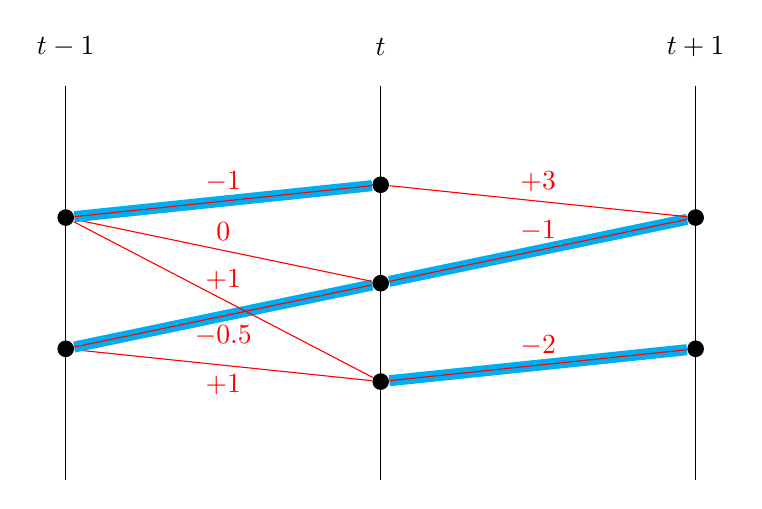
\begin{tikzpicture}
      \draw (0,0) -- (0,5);%
      \draw (4,0) -- (4,5);%
      \draw (8,0) -- (8,5);%

      \node[circle,inner sep=0pt, minimum size=6pt,fill] (A1) at (0,1.6666) {};%
      \node[circle,inner sep=0pt, minimum size=6pt,fill] (A2) at (0,3.3333) {};%

      \node[circle,inner sep=0pt, minimum size=6pt,fill] (B1) at (4,1.25) {};%
      \node[circle,inner sep=0pt, minimum size=6pt,fill] (B2) at (4,2.5) {};%
      \node[circle,inner sep=0pt, minimum size=6pt,fill] (B3) at (4,3.75) {};%

      \node[circle,inner sep=0pt, minimum size=6pt,fill] (C1) at (8,1.6666) {};%
      \node[circle,inner sep=0pt, minimum size=6pt,fill] (C2) at (8,3.3333) {};%

      \draw[red] (A1) -- (B1) node[midway,below] {$+1$};%
      \draw[red,preaction={ draw,cyan,-,double=cyan, double
        distance=8\pgflinewidth, }] (A1) -- (B2) node[midway,below] {$-0.5$};%
      \draw[red] (A2) -- (B1) node[midway,above] {$+1$};%
      \draw[red] (A2) -- (B2) node[midway,above] {$0$};%
      \draw[red,preaction={ draw,cyan,-,double=cyan, double
        distance=8\pgflinewidth, }] (A2) -- (B3) node[midway,above] {$-1$};%

      \draw[red,preaction={ draw,cyan,-,double=cyan, double
        distance=8\pgflinewidth, }] (B1) -- (C1) node[midway,above] {$-2$};%
      \draw[red,preaction={ draw,cyan,-,double=cyan, double
        distance=8\pgflinewidth, }] (B2) -- (C2) node[midway,above] {$-1$};%
      \draw[red] (B3) -- (C2) node[midway,above] {$+3$};%

      \node at (0,5.5) {$t-1$};%
      \node at (4,5.5) {$t$};%
      \node at (8,5.5) {$t+1$};%
    \end{tikzpicture}
    \caption{Matching detections only in pairs of frames. The results are not
      consistent across frames.}
  \end{subfigure}
  \begin{subfigure}{\textwidth}
    \centering
    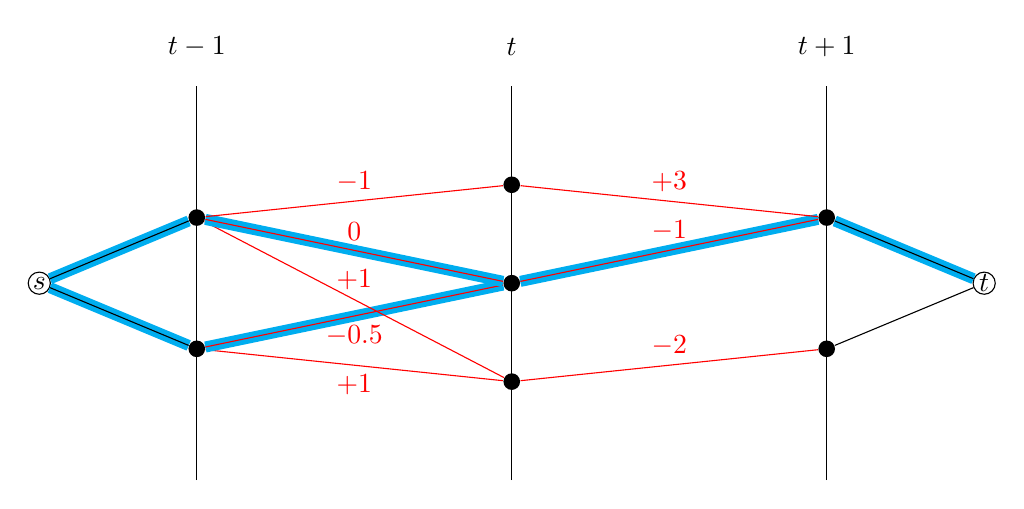
\begin{tikzpicture}
      \draw (0,0) -- (0,5);%
      \draw (4,0) -- (4,5);%
      \draw (8,0) -- (8,5);%

      \node[circle,inner sep=0pt, minimum size=6pt,fill] (A1) at (0,1.6666) {};%
      \node[circle,inner sep=0pt, minimum size=6pt,fill] (A2) at (0,3.3333) {};%

      \node[circle,inner sep=0pt, minimum size=6pt,fill] (B1) at (4,1.25) {};%
      \node[circle,inner sep=0pt, minimum size=6pt,fill] (B2) at (4,2.5) {};%
      \node[circle,inner sep=0pt, minimum size=6pt,fill] (B3) at (4,3.75) {};%

      \node[circle,inner sep=0pt, minimum size=6pt,fill] (C1) at (8,1.6666) {};%
      \node[circle,inner sep=0pt, minimum size=6pt,fill] (C2) at (8,3.3333) {};%

      \node[draw,circle,inner sep=0pt, minimum size=8pt] (S) at (-2,2.5) {$s$};%
      \node[draw,circle,inner sep=0pt, minimum size=8pt] (T) at (10,2.5) {$t$};%
      
      \draw[red] (A1) -- (B1) node[midway,below] {$+1$};%
      \draw[red,preaction={ draw,cyan,-,double=cyan, double
        distance=8\pgflinewidth, }] (A1) -- (B2) node[midway,below] {$-0.5$};%
      \draw[red] (A2) -- (B1) node[midway,above] {$+1$};%
      \draw[red,preaction={ draw,cyan,-,double=cyan, double
        distance=8\pgflinewidth, }] (A2) -- (B2) node[midway,above] {$0$};%
      \draw[red] (A2) -- (B3) node[midway,above] {$-1$};%

      \draw[red] (B1) -- (C1) node[midway,above] {$-2$};%
      \draw[red,preaction={ draw,cyan,-,double=cyan, double
        distance=8\pgflinewidth, }] (B2) -- (C2) node[midway,above] {$-1$};%
      \draw[red] (B3) -- (C2) node[midway,above] {$+3$};%

      \draw[black,preaction={ draw,cyan,-,double=cyan, double
        distance=8\pgflinewidth, }] (S) -- (A2);%
      \draw[black,preaction={ draw,cyan,-,double=cyan, double
        distance=8\pgflinewidth, }] (S) -- (A1);%

      \draw[black] (C1) -- (T);%
      \draw[black,preaction={ draw,cyan,-,double=cyan, double
        distance=8\pgflinewidth, }] (C2) -- (T);%
      
      \node at (0,5.5) {$t-1$};%
      \node at (4,5.5) {$t$};%
      \node at (8,5.5) {$t+1$};%
    \end{tikzpicture}
    \caption{Matching detections using the shortest path and second shortest
      path. A single edge is used more than once what is not desired.}
  \end{subfigure}
  \caption{Example for tracking without division.}%
  \label{fig:tracking}
\end{figure}


                                     
%%% Local Variables:
%%% mode: latex
%%% TeX-master: "../main"
%%% End:
